\chapter{Introduction}

This chapter will introduce the notion of rephotography, elaborate on the
process of how to make such a photograph and survey existing approaches to
simplify it. These include two applications for mobile operating systems which
will be briefly discussed. Furthermore, a summary of more sophisticated work by
MIT researchers will be given, leading to the problem statement and the goal of
this work.

\section{Rephotography}

\emph{Rephotography} or repeat photography denotes the retrieval of the precise
viewpoint used for taking a---possibly historic---photograph and capturing
another image from the same spot, ideally with the same camera parameters. This
allows for documentation and visualisation of changes which the scene has
undergone between the two or more captures.  For instance when documenting urban
development, one can present progress of construction, restoration efforts or
changes in the surroundings in a visually striking manner, e.g. by blending the
photographs together.  Figures \ref{fig1} and \ref{fig2} show examples.

\begin{figure}
   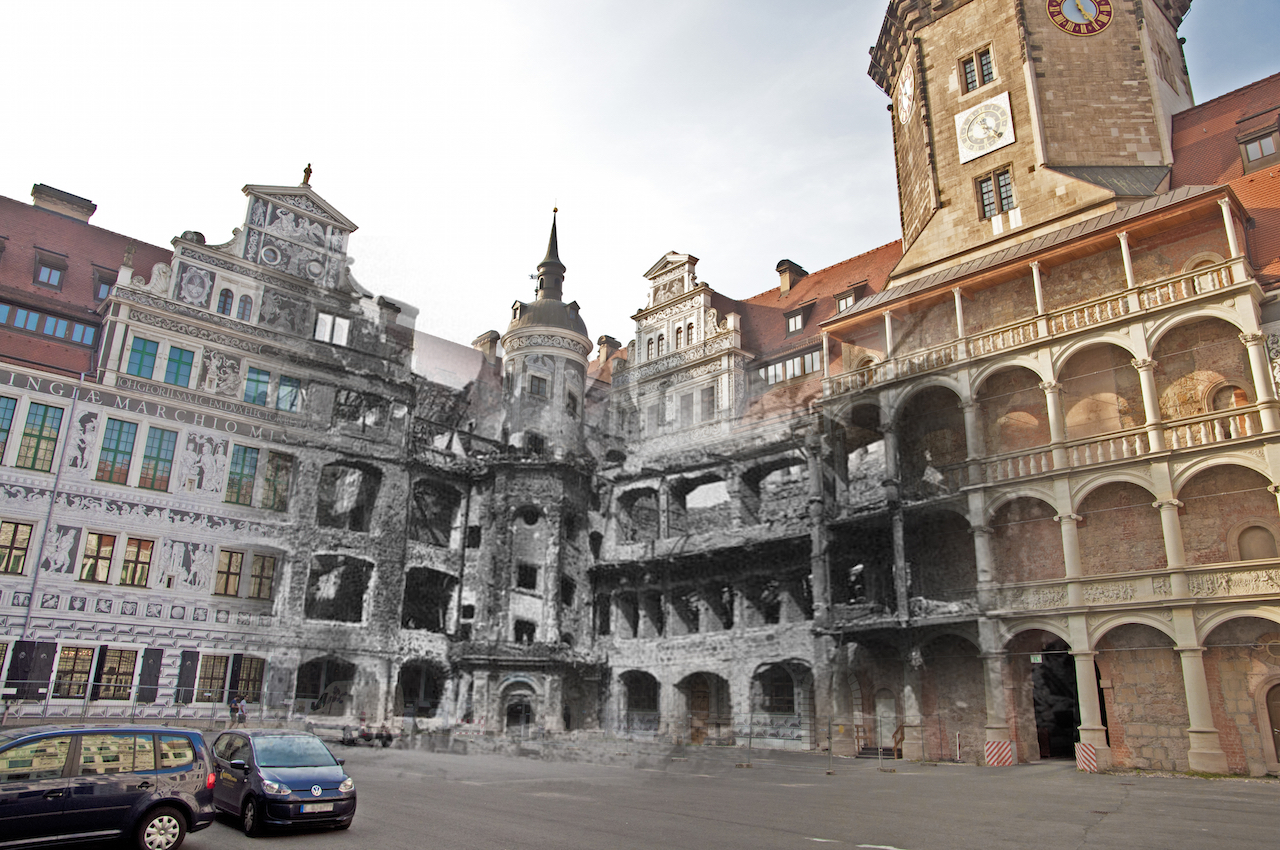
\includegraphics[width=\textwidth]{gfx/1945_2014_Residenzschloss_small.jpg}
   \caption[Rephoto of Dresden Castle]{Rephoto of the Dresden Castle, destroyed during World War II,
   \textcopyright\ Sergey Larenkov, printed with permission}
   \label{fig1}
\end{figure}

\begin{figure}
   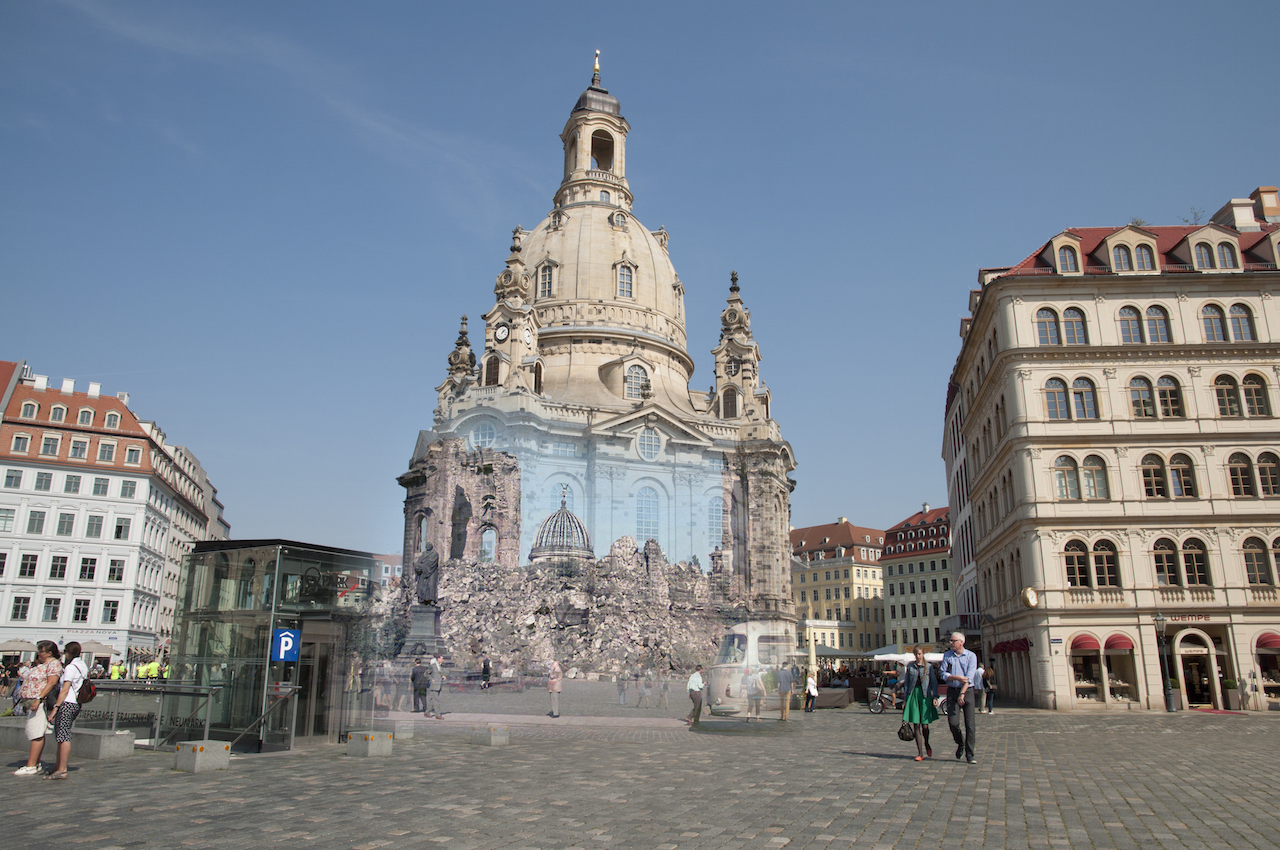
\includegraphics[width=\textwidth]{gfx/1950_2014_Frauenkirche_small.jpg}
   \caption[Rephoto of Dresden Frauenkirche]{Rephoto of the Dresden Frauenkirche, destroyed during World War II,
   \textcopyright\ Sergey Larenkov, printed with permission}
   \label{fig2}
\end{figure}

When done manually, the photographer must attempt to find the original viewpoint 
usually by visual inspection of the original image and trying to match the
current camera parameters---camera position, camera rotation, focal length,
possibly principal point---to the original.
The procedure is often carried out by placing the camera on a tripod and
comparing a printout of the original image with what can be seen through the
viewfinder or the camera screen. The number of parameters to match as well as
the difficulty to estimate them purely from comparing two-dimensional images makes the process
error-prone and tedious. Visual acuity and experience of the photographer thus
place limits on the accuracy with which the camera pose of the reference image
can be reconstructed. Some corrections can be done by post-processing the images
and warping the rephotograph with a homography to better match the original, but
it would be preferable to achieve a good result in-camera.

At the time of writing, few computerised aids are available to the photographer
(see \autoref{subsec:mobile_apps}).  The advancement of mobile phones and tablet
computers with integrated cameras and larger screens presents the opportunity to
develop applications which can assist in this endeavour, moving away from the
traditional trial-and-error approach.  On current digital cameras\footnote{At
   the time of writing, no commercial manufacturer produces a camera with
   user-modifiable firm- or software. A project at Stanford by \citet{Levoy2010}
was discontinued \citep{FrankenCam}.} this is impossible due to their closed
infrastructure not permitting to run user programs. 

\section{Previous Approaches To Assisted Rephotography}

\subsection{Mobile Applications}\label{subsec:mobile_apps}

Two applications have been developed to assist a photographer in taking
rephotographs. For smartphone operating systems,
\emph{rePhoto}\footnote{\url{http://projectrephoto.com/}} and
\emph{Timera}\footnote{\url{http://www.timera.com/Explore}} exist, both
available for Android and iOS devices. These applications support the user by placing a transparent
version of the original image over the current camera image, allowing for easier
alignment. 
Both apps present the captured rephoto with the original image blended in, but
only Timera allows for customisation (see \autoref{fig:timera})

What is characteristical about both of these applications is that the user must still
determine on their own how to actually move the camera. An overlay simplifies
the procedure, eliminating some of the inaccuracy introduced into the manual approach by the
necessity to move the eyes from printout to camera, but it is still the user's
responsibility to determine the necessary motion between the current camera
position and the goal position (that of the original image). 

\subsection{Computational Re-Photography}

A more sophisticated automated approach was presented by \citet{bae2010}. They
found in preliminary studies that neither a side-by-side view, as would be used
in the manual approach, nor a linear blend provided by the above applications
result in accurate rephotographs. Their design applies image processing and
geometrical reconstruction of the scene in order to guide the user into the right direction.

In this setup, the relevant parameters of a historic image's camera are
reconstructed, including the focal length, principal point and the six degrees
of freedom in camera pose with structure-from-motion (SfM) techniques. This
subsection will give a brief overview, while a more in-depth discussion of the
relevant concepts is deferred to \autoref{sec:app_challenges}. Five problems
are addressed by \citet{bae2010}.

\begin{enumerate}
   \item It is difficult to communicate a necessary motion to the user if it has
      six degrees of freedom .
   \item While it is possible to compute the direction of translation between
      two camera frames given some corresponding points, its scale is unknown so
      that one does not know how far to move.
   \item As the translation between two camera frames becomes small, the
      estimate of relative translation becomes unstable.
   \item Historic images are visually very different from current ones, so that
      automatic feature detection will not work.
   \item The historic images' camera is unknown, but its calibration parameters
      (see \autoref{subsec:intrinsics}) are needed.
\end{enumerate}

To solve these problems, \citet{bae2010} have the user capture two frames of the
scene with a wide baseline. Manual selection of some correspondences between the
historic images and one of the two just taken eliminates the fourth problem,
while the second one can be addressed by using the two images and the current
camera frame for 3D reconstruction. To ease the user's task, the current camera
image is warped according to the camera rotation relative to the reference imge.
The user can then
focus on correctly translating the camera. The fifth problem is solved by
estimating the parameters after the user has identified some lines in the image
which are parallel in reality.

The software runs on a laptop connetcted to a digital camera. On the computer
screen, the user is shown the current camera image alongside two arrows
indicating in which direction to move---one for movement in the sensor plane and
one for movement along the optical axis.

The results of this method appear to be very successful, but two main drawbacks
exist.

\begin{itemize}
   \item The prototype is not very convenient, as it requires a (laptop)
      computer and a digital camera which is impractical for
      spontaneous rephotography.
   \item The application is not available to the public, neither in source nor
      binary form. It is therefore impossible to evaluate or adapt for more mobility.
\end{itemize}

\section{Goals of this thesis}

This work's objective can thus be summarised as follows.
\begin{enumerate}
   \item Implement in a prototypal fashion the process from \citep{bae2010} for
      a mobile operating system so it can be run on a smartphone or tablet and
      direct the user in approximate real-time.
   \item Evaluate the approach and attempt to reproduce the results.
\end{enumerate}

For a proof-of-concept application, several simplifying assumptions are made.
Firstly, it is assumed that the ``historic'' photograph is captured with the
same camera as the one running the application and that the camera is calibrated.
Secondly, no strong visual differences between the reference and current scenes
are assumed so that the reference image is accessible to the same feature
detection algorithm without the user manually labelling correspondences. 

The application targets iOS 8 and current hardware, as image processing is
computationally intense, and has been tested on an iPad Air 2.
